\documentclass[preprint,12pt]{article}

\usepackage{algorithmic}
\usepackage{algorithm}
\usepackage{enumerate}
\usepackage{enumitem}
\usepackage{graphics}
\usepackage{graphicx}
\usepackage{geometry}
\usepackage{amsmath}
\usepackage{wrapfig}
\usepackage{subfig}
\usepackage{framed}
\usepackage{color}
\usepackage{soul}
\usepackage{bm}

\usepackage{natbib}
\usepackage{multirow}
\usepackage[T1]{fontenc}
\usepackage[latin9]{inputenc}
%\usepackage{units}
\usepackage{esint}
\geometry{legalpaper,  margin=1in}

\newcommand{\CM}[2][green]{ {\sethlcolor{#1} \hl{#2}} }
\newcommand{\KB}[2][cyan]{ {\sethlcolor{#1} \hl{#2}} }
%THIS IS TO PUT ALL FLOATS AT THE END OF THE DOC SO THEY CAN BE SPLIT INTO A SEPARATE FILE
%%\usepackage{endfloat}
%\makeatother

%\usepackage{babel}

\begin{document}
\title{Some Thoughts on Mean - Median}


\maketitle

\begin{abstract}
The mean median difference test is an attractive gerrymandering standard for many reasons.
It meets constitutional requirements and is arguably the simplest metric to calculate and conceptualize.
While it does not work for states that are not close to even partisanship, the worst gerrymandering occurs in close states.
These states are also of high strategic value for those seeking to take control of a statehouse in advance of redistricting.

Here we consider two issues related to the test, namely whether the standardized or unstandardized mean median difference should be used, and whether the sampling variance of mean median difference should be estimated from historical data or using the asymptotic variance from an assumed null distribution.

\end{abstract}

\section{Introduction}
The mean median difference test \cite{Wang__,Wang_2016_10.1089/elj.2016.0387,McDonald_2015_10.1089/elj.2015.0358}, fits with existing rulings since it measures partisan bias without regard to proportionality and is simple enough to be calculated by a judge without an expert witness.
While it is only effective in measuring bias for states which are close to even in terms of partisanship, \cite{Wang_2016_10.1089/elj.2016.0387}, close states account for a major portion of the gerrymandering that occurs in the US.
The mean median difference statistic can be standardized or unstandardized. 
We denote these two statistics as $C_{s}$ and $C_{u}$ respectively, and they are defined as follows
\begin{equation}
    C_{s} = \frac{\bar{X}-\theta}{S}
\end{equation}

\begin{equation}
    C_{u} = \bar{X}-\theta
\end{equation}
Where $\bar{X}$ is the mean district vote percentage, $\theta$ is the median district vote percentage, and $S$ is the standard deviation of the district vote percentages.
The standardized statistic $C_{s}$ is therefore simply $C_{u}$ divided by the standard deviation.

In section \ref{sec:var}, we consider how the variance for estimating p-values of these statistics should be calculated.
Wang has proposed the asymptotic variance for a unit normal distribution for $C_{s}$, which was derived by \cite{Cabilio_1996_10.2307/3315744}.
Similar calculations for $C_{u}$ can be found in \cite{Cabilio_1996_10.2307/3315744} and \cite{Mira_1999_10.1080/02664769921963}.
We consider two separate but related aspects of this.
First, if we accept the assumption of independent and identically distributed districts that is required for deriving an asymptotic variance, then what is the most appropriate null distribution to use?
Second, we consider whether an asymptotic variance should be used with a null distribution at all.
Districts vote percentages are neither independent nor identically distributed, but a normal distribution is still a reasonable assumption for the sampling distribution of $C_{s}$ and $C_{u}$.
As an alternative to an asymptotic variance, we estimate the variance using an empirical Bayesian simulation.

In section \ref{sec:gaming}, we will show that $C_{u}$ is preferable since $C_{s}$ allows bad actors to manipulate the standard by increasing the standard deviation of the district vote percentages.
Not only does this allow gerrymanderers to skirt a potential standard based on $C_{s}$, but it provides an incentive for them to create even more polarized districts, which is the result of increasing the standard deviation of district voter percentages.
In contrast, $C_{u}$ can not be manipulated in the same fashion.


\section{The Sampling Variance\label{sec:var}}

For a continuous symmetric distribution with density function $f$, mean $\mu$, variance $\sigma^{2}$, and median $\nu$, the asymptotic sampling variances $\sigma^{2}_{s}$ and $\sigma^{2}_{u}$ for $\sqrt{n}C_{s}$ and $\sqrt{n}C_{u}$ respectively are \cite{Cabilio_1996_10.2307/3315744,Mira_1999_10.1080/02664769921963}.

\begin{equation}
    \sigma^{2}_{s} = 1 +\frac{1}{4\sigma^{2}f^{2}\left(\nu\right)}-\frac{\tau}{\sigma f\left(\nu\right)}
\end{equation}
and
\begin{equation}
    \sigma^{2}_{u} = \sigma^{2} +\frac{1}{4f^{2}\left(\nu\right)}-\frac{\tau}{f\left(\nu\right)}
\end{equation}
where 
\begin{equation}
    \tau = \mu - 2\int_{-\infty}^{\nu} xf\left(x\right)dx
\end{equation}
These variances can be computed readily for common symmetric distributions, but can additionally be estimated from data by using a kernel density estimate of the data and numerical quadrature to approximate the above integrals.
The asymptotic variance for the unit normal distribution is used quite commonly and proposed by Wang for use as a gerrymandering standard, but other distributions can be considered as well to try to better reflect voting data in actual elections. In addition we consider a uniform distribution on the unit interval, a uniform distribution on the interval .15 - .85, and a KDE estimate of all contested elections in US congress from 1972-2016, symmetrized about 0.5.
The variances are tabulated in table \ref{tab:var} and KDE estimate for the voting data is in figure \ref{fig:kde}.

\begin{table}[htb!]
\centering
\caption{Asymptotic variances for $C_{u}$ and $C_{s}$ for a few distributions \label{tab:var}}
\begin{tabular}{|l|l|l|}
\hline
Distribution & $\sigma^{2}_{s}$ & $\sigma^{2}_{u}$\\
\hline
\hline
Unit Normal & 0.5708 & 0.5708\\
\hline
Uniform (0,1) & 1.0 & 0.0833\\
\hline
Uniform (0.15,0.85) & 1.0 & 0.0408\\
\hline
Symmetrized Voting Data & 1.2022 & 0.0395\\
\hline
\end{tabular}
\end{table}

\begin{figure}[htb!]
    \begin{center}
        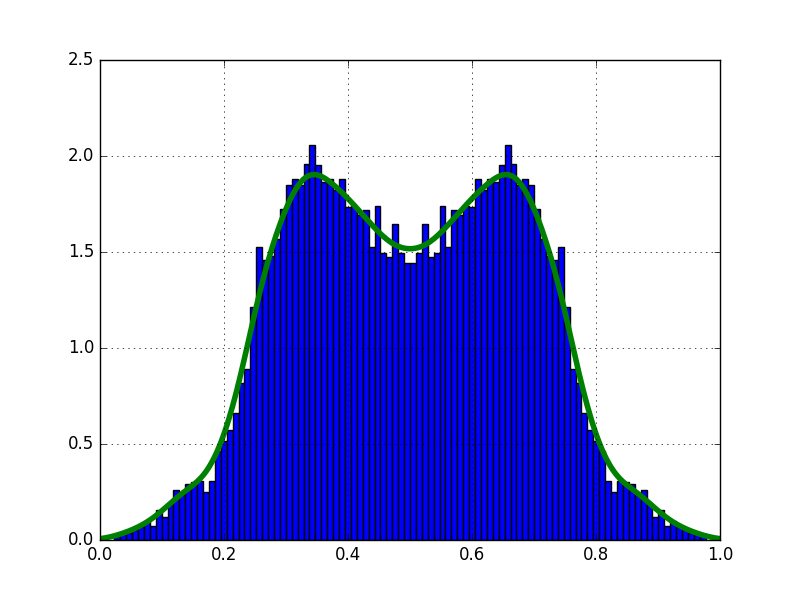
\includegraphics[scale=0.8]{../Figures/SimVsAsymptotic/Kde.png}
        \caption{Histogram and KDE estimate of symmetrized voting data}\label{fig:kde}
    \end{center}
\end{figure}

An alternative procedure for estimating these variances is to simulate elections and compute the variance of $C_{u}$ and $C_{s}$ from the result.
This is done by estimating a beta distribution for each district using the method of moments and a hyperprior for the variance, and simulating 10,000 elections.
This removes the assumption of identically distributed districts and also removes the discrepancy between the asymptotic and actual sampling variance at small sample sizes.
The sampling variances are then estimated by computing the variance that best fits the simulated variances.
While the mean median difference is only effective for measuring gerrymandering for close states, here we are only interested in the variance of the statistic from election to election so close states and partisan states are both included in the fit.
Plots are shown in figures \ref{fig:sCs} and \ref{fig:sCu}, and the results of fitting are 0.2345 for $C_{s}$ and 0.0057 for $C_{u}$.
Both of these are substantially smaller than the asymptotic results from table \ref{tab:var}, although for $C_{s}$ the standard normal variance seems like a reasonable high end estimate.
Additionally for $C_{s}$ the smallest possible asymptotic variance for a unimodal distribution is 0.25.
These results suggest that the sampling variance of the mean median difference, regardless if it is standardized or not, should be estimated from historical data rather than an asymptotic variance from some null distribution.
The method used here combines historical data with an empirical model, but that is not the only possibility.
More sophisticated models could be used, or no model could be used at all, and the sampling variance could be estimated directly from the data.


\begin{figure}[htb!]
    \begin{center}
        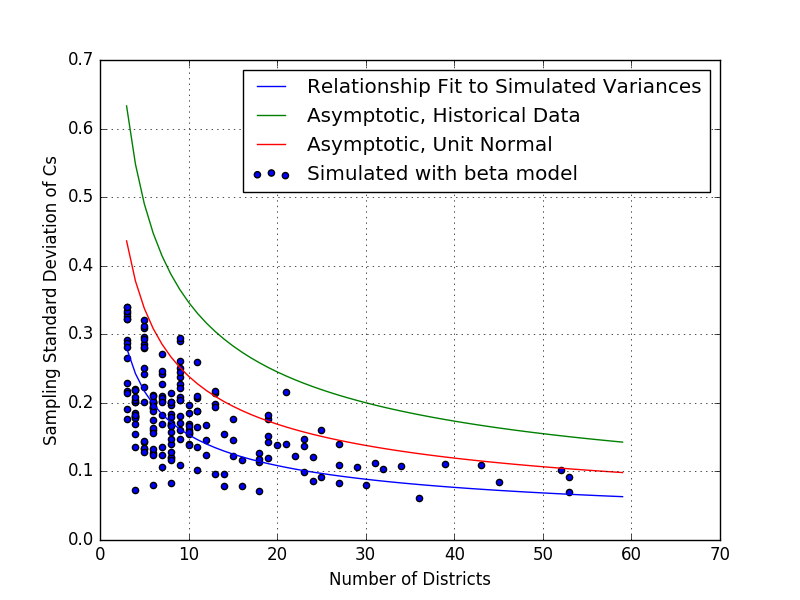
\includegraphics[scale=0.8]{../Figures/SimVsAsymptotic/stdv_nCs.png}
        \caption{Asymptotic and fit variances for the standardized mean median difference}\label{fig:sCs}
    \end{center}
\end{figure}

\begin{figure}[htb!]
    \begin{center}
        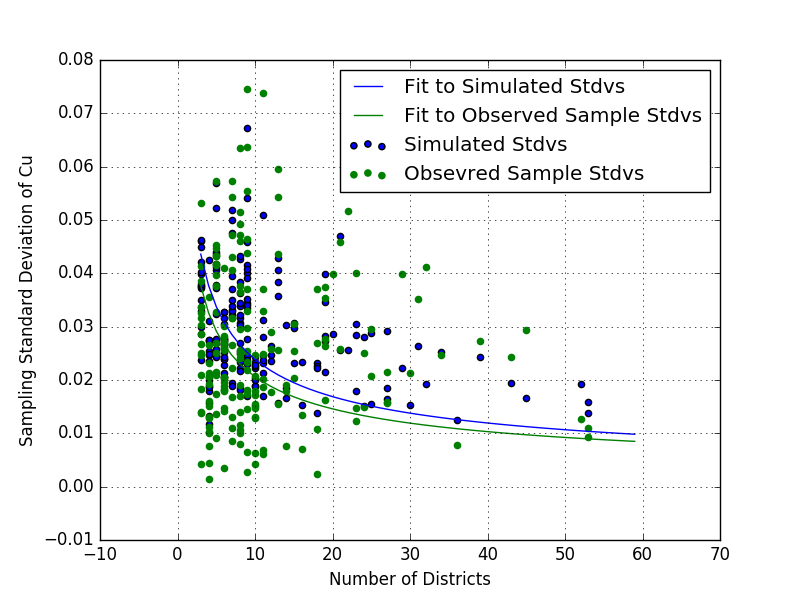
\includegraphics[scale=0.8]{../Figures/SimVsAsymptotic/stdv_nCu.png}
        \caption{Asymptotic and fit variances for the unstandardized mean median difference}\label{fig:sCu}
    \end{center}
\end{figure}


\section{Gaming the Mean Median Difference\label{sec:gaming}}
The adoption of any standard to reign in gerrymandering will lead to attempts to skirt around it.
One approach to gaming $C_{s}$ is to simply increase the standard deviation of the district vote percentages, which decreases the p-value of the test.
This can be done while keeping $C_{s}$ essentially unchanged.
To illustrate this, we use a multi objective optimization technique, where we minimize the district standard deviation while maximizing the p-value for $C_{s}$ using the asymptotic variance from the unit normal.
We use 18 districts and require that one party get at least 14 safe wins, where a safe win is defined as having at least 55\% of the vote.
The mean of the district votes must lie within 0.5\% of 50.0\%, and the vote percentages in any district must be within 15\% and 75\%.
At some point, decreasing the district standard deviations must come at the expense of also decreasing the p-value of the test.
This results in a family of non dominated or Pareto optimal solutions representing the trade off between these two objective.
The reason for this procedure is to show how $C_{s}$ can be gamed solely by changing the standard deviation as opposed to some combination of changing $C_{u}$ as well as the standard deviation, since we will look at attempting to game $C_{u}$ in a moment.
\begin{figure}[htb!]
    \begin{center}
        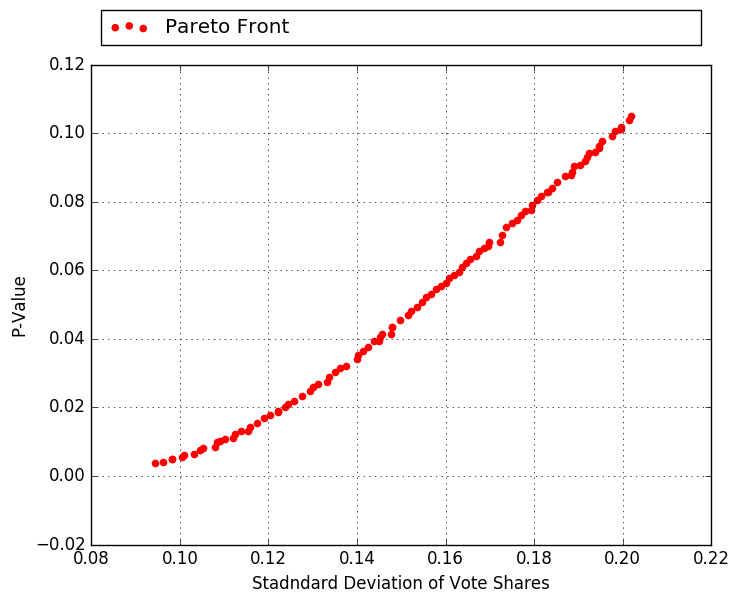
\includegraphics[scale=0.8]{../Figures/SimVsAsymptotic/pareto.png}
        \caption{Pareto front for gaming the standardized mean median difference}\label{fig:pareto}
    \end{center}
\end{figure}

Figure \ref{fig:pareto} shows the resulting Pareto front, and under the assumptions of this simple analysis, it is possible to safely win 14 of 18 seats (77.8\%) safely with 50\% of the vote while manipulating $C_{s}$ to obtain a p-value above the usual threshold of 5\%.
Further, in each of the Pareto optimal solutions the mean median difference is essentially the same.
This is shown in figure \ref{fig:solutions}, where each pareto optimal solution for the vote percentages is plotted.
Is a different sampling variance was adopted on the basis of the results of section \ref{sec:var}, then this would improve the situation somewhat since the resulting standard would be stricter, but this change alone would not resolve the vulnerability of $C_{s}$ based standards.

\begin{figure}[htb!]
    \begin{center}
        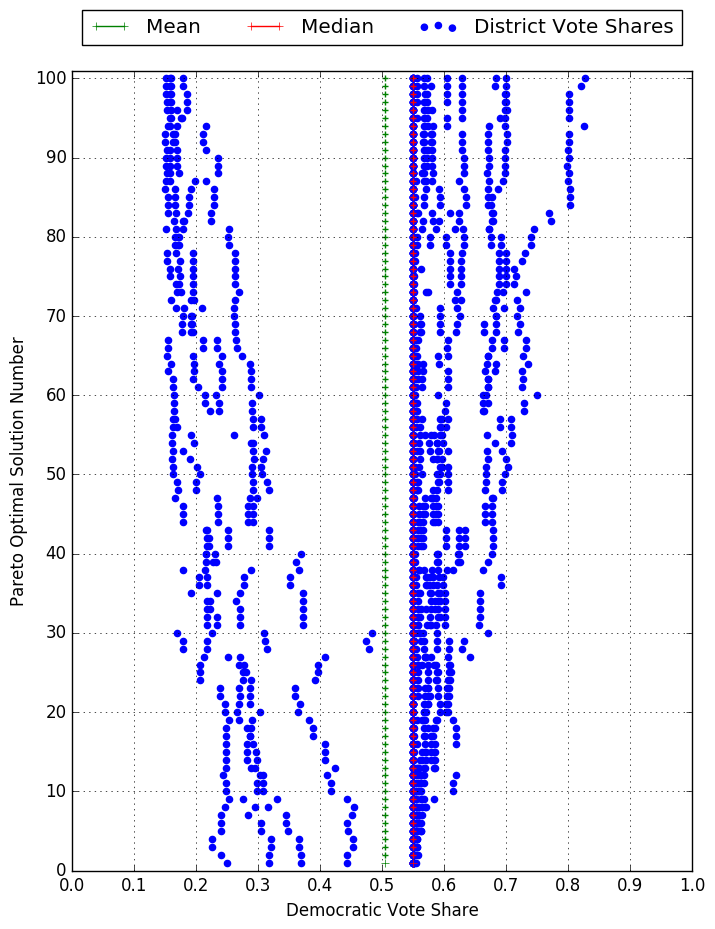
\includegraphics[scale=0.8]{../Figures/SimVsAsymptotic/solutions.png}
        \caption{Pareto optimal solutions shown in each row of the plot. As the rows move up from the bottom the p-value of the test increases along with the standard deviation of the vote percentages}\label{fig:solutions}
    \end{center}
\end{figure}

It is also evident that if the gerrymanderers were forced to reduce $C_{u}$ then this would require them to either give up some of their safe wins or lower their safe win threshold from 55\% to something lower.
This is what we want, since it results in less bias and more competition in the state's elections.
To illustrate this we again use optimization, but with a slightly different approach from before.
Instead of multiobjective optimization, we do a series of single objective optimizations with different numbers of safe wins and safe win thresholds while trying to maximize the p value of the $C_{u}$ test using the sampling variance from the previous section.
For 18 seats, only 9 safe wins could be achieved while passing the test for $C_{u}$ with a safe win threshold of 55\%.
In order to achieve more than 9 safe wins while passing the test, the safe win threshold would need to be reduced, making those wins less secure.
This is shown in figure \ref{fig:sw}

\begin{figure}[htb!]
    \begin{center}
        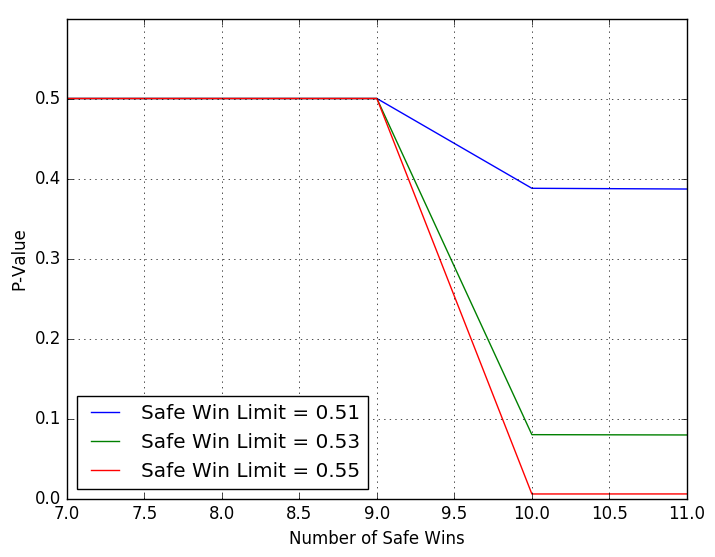
\includegraphics[scale=0.8]{../Figures/SimVsAsymptotic/gamingCu.png}
        \caption{Number of achievable save wins for different safe win thresholds}\label{fig:sw}
    \end{center}
\end{figure}
\section*{Acknowledgment}
\section*{}
\bibliographystyle{unsrt}
\bibliography{gerrymandering}
\clearpage



\end{document}
